%%% Research Diary - Entry
%%% Template by Mikhail Klassen, April 2013

\documentclass[11pt,letterpaper]{article}

\newcommand{\workingDate}{\textsc{2022 $|$ January $|$ 31}}
\newcommand{\userName}{Ganning Xu}
\newcommand{\institution}{Research in \\ Computational Science \\ North Carolina School of Science and Math}
\usepackage{researchdiary_png}
%\usepackage{natbib}
%\bibliographystyle{abbrvnat}
%\setcitestyle{authoryear,open={((},close={))}}
\usepackage{float}
\usepackage{wrapfig}
\usepackage{hyperref}
\usepackage{hyperref}

\begin{comment}
Resources
    Table Generator: https://www.tablesgenerator.com/
    Overleaf Project: https://www.overleaf.com/project/61fc1906472d003c89b4c1f1
    GitHub Project: https://github.com/ganning127/RCompSci_Research_Notebook
\end{comment}

\begin{document}
\univlogo

\section{Week of January 31, 2022}

$\surd$ {\Large \textcolor{red}{RRG Comment:acknowledging notebook establishment } } 

\textbf{Note}: I take a lot of my notes in my \href{https://drive.google.com/drive/folders/17ZhkJZveiDomM2K2MYST_-PhuzrndiVT?usp=sharing}{Google Drive}, so my notebook might not be as detailed.

\subsection{Monday, January 31, 2022}
First day of research in computational science. Went over introductions, course expectations, and how this class would work.

\subsection{Wednesday, February 2, 2022}
Went over how to read request for proposals (RFP) and covered the Research in Computational Science \href{https://drive.google.com/file/d/1cvPQnz40H3bqiEyOdgzRMyYjtK4gxPB5/view?usp=sharing}{RFP}.


We also covered an intro \href{https://drive.google.com/file/d/1hlGEsI95i6WEo5NzAbqjr73ax-MP5L8G/view?usp=sharing}{guide to computational thinking}. Begin by starting with a research question that can be broken down into subproblems. The first subproblem should be "low hanging fruit", while the latter ones should be harder to achieve. Also, it is important to make assumptions when creating the model, as it simplifies it. It's important to be able to distinguish which data is important and which data is not as useful. 

When creating algorithms, you can either use an existing one, modify an existing one, or create your own. Creating your own algorithm is usually difficult. 

\textbf{Important notes}
\begin{itemize}
    \item Letter of intent due on Friday, March 4, 2022 at 5 PM. 
    \item Preliminary proposal due on Friday, March 25, 2022, at 5 PM. 
    \item Full proposal due Wednesday, April 20, at 5 PM. 
\end{itemize}

\subsection{Thursday, February 3, 2022}
Learned \LaTeX 

Table \ref{tab:ideas} shows a table of some of my ideas for my research work.

\begin{table}[H]
\begin{center}
\begin{tabular}{|c|c|c|c|}
\hline
\textbf{Topic idea} & \textbf{\begin{tabular}[c]{@{}c@{}}Technology\\ Computational "X"\end{tabular}} & \textbf{Techniques and Tools} \\ \hline
Heart disease detection algorithm & Machine Learning & TensorFlow, Keras, Kaggle \\ \hline
Long text simplification & NLP & GTP3 and Kaggle \\ \hline
Factors of a successful election & Machine Learning & TensorFlow, Keras, Large dataset \\ \hline
\end{tabular}
\caption{Table of CT Ideas}
\label{tab:ideas}
\end{center}
\end{table}

\subsection{Friday, February 4, 2022}

\subsubsection * {How Science Works}
Today we learned about how science works from the national level to a researcher when they submit their RFP. Here is a link to my \href{https://docs.google.com/document/d/17-9rgkjDyZuy95PmMjWT7NfPlYd96HXTcVR5unhhW_A/edit?usp=sharing}{notes}. 

Basically, the flow of power works like this: NSB $\rightarrow$ NSF $\rightarrow$ Directorates $\rightarrow$ Groups $\rightarrow$ RFP. 

Once a researcher sends in an RFP:
\begin{enumerate}
    \item The RFP is sent to a specific project officer (typically university faculty on loan)
    \item The Project Officer will then create a certain number of review teams (~5 in team team), to review ~20 proposals.
    \item Each person in a review team scores each proposal (excellent, very good, good, fair, poor)
    \item After individual review, each review team goes to Washington DC and works on reviewing proposals for ~3 days in a review panel together
    \item Each proposal is ranked into (High, medium, and low) priority for funding. This recommendation goes to the NSF project officer, who makes a decision on who gets the money. They can overrule a panel.
\end{enumerate}

When an RFP is approved, the person in charge of the research is the Principal Investigator (PI). Each PI usually has CoPI's, unless the project is really small. 

\subsubsection * {Example RFP}
Today, we also looked over an example RFP that Mr. Gotwals submitted. It is important to note that the project summary can only be one page long and the project description has to be less than 15 pages. 

\subsection{Saturday, February 5, 2022}
Today I read over the example proposal that Mr. Gotwals gave us and completed the reading check that covered the podcast and the Intro to Computational Thinking chapter. I also started on the content from the proposal template today.

\subsection{Sunday, February 6, 2022}
Read over \href{https://drive.google.com/file/d/1weJUCV1x84bmy6dvqFjRlOviiD8dVDjg/view?usp=sharing}{GotwalsGuideCT.pdf}. Also read over \href{https://drive.google.com/file/d/1p4ew41jI2WH81WCaB8ADkFOrTVsac7Wl/view?usp=sharing}{How to summarize a research paper}.

\section{Week of February 7, 2022}
\subsection{Monday, February 7, 2022}
Learned about how spreadsheets worked in class. Completed three spreadsheet labs from the Bohr model, Gaussian Distribution, and Diatomic molecules. 

\subsection{Tuesday, February 8, 2022}
Corrected one of the spreadsheet labs.

\subsection{Wednesday, February 9, 2022}
\href{https://www.ncssm.edu/library}{ncssm.edu/library} is a good source for research articles. The \href{https://ncssm.follettdestiny.com/common/servlet/presenthomeform.do?l2m=Home&tm=Home&l2m=Home}{full catalog} has acess to journals.

\begin{itemize}
    \item HeinOnline - Legal
    \item Liebert Medical Journals - Medical Research
    \item JSTOR - Humanities
    \item NC Live - Biggest DB (UNC System, private colleges, community colleges). Can access the NYTimes and Washington post through here
\end{itemize}

\textbf{Ways to read a research paper}
\begin{enumerate}
    \item Read abstract and conclusions. If important can look at the entire thing. 
    \item The last sentence of the introduction usually contains the RQ
    \item Look at references of research paper first (see if you see a certain name that is repeated, they are the expert)
    \item Read many papers from the expert and see if you can reach out to them for them to be your mentor
    \item Keep the \href{https://www.mendeley.com/reference-manager/}{citation manager} UPDATED!
\end{enumerate}

\textbf{Types of Research}
\begin{itemize}
    \item Literature Review: A researcher goes out and finds research papers about a topic over a certain period of time. This is very good to find if you can. 
\end{itemize}


\subsection{Thursday, February 10, 2022}
Today I read over the research paper: Recent Approaches for Text Summarization Notes, and created a draft of my J-Club presentation on the topic. There are two main types of text summarization: abstractive and extractive. Abstractive summarization focuses on semantic understanding the text and re-expressing that understanding in easier words. Extractive summarization focuses on removing unnecessary sentences and words to create a summary sentence with parts of existing ones.

\subsection{Friday, February 11, 2022}
Today was the Mathematica lab, where we learned how to perform text analysis on a speech that was 80,000 characters long. I also made edits to my J-Club draft today.

\subsection{Saturday, February 12, 2022}
I was at the NCHSAA States Swim meet for today, so I didn't get a chance to work on RCompSci.

\subsection{Sunday, February 13, 2022}
Today I read over my research paper for JClub again and took more notes on it. I think that I have a good idea of how I'm going to do my JClub presentation.

\section{Week of February 14, 2022}
\subsection{Monday, February 14, 2022}
Today I worked on my JClub presentation: Shortening sentences, including graphics with captions, and making sure that I truly understood everything that I will be talking about. However, this was difficult as the paper I read had some complicated math in it and a LOT of grammatical errors. I finished the draft of my JClub presentation today.

Today I also created a script that I will be using to practice for my JClub presentation.

\subsection{Tuesday, February 15, 2022}
I read over the "Top60QuestionsFrequentlyAskedDuringThesisDefense.pdf" and "rocreguant.com-What questions to ask after a scientific presentation.pdf" files on Canvas. While asking questions may seem like you're hassling the researcher, in reality, you're actually helping them see their own project from another perspective, something different from what they're used to. Some good questions:

Make sure to always be polite when asking questions.
\begin{itemize}
    \item What is next for your research project?
    \item The results of your findings seem promising, but they contradict X, why is this?
\end{itemize}

Additionally, I learned that you should never actually show the true weaknesses of the research project you are "defending". You don't want to give the other side any doubts of uncertainty. 

Today I also made edits to my JClub presentation and edited my script to make sure that there were no typos.

\subsection{Wednesday, February 16, 2022}
Today I read over the ATE RFP and a sample proposal and completed the proposal review guide. I realized that:
\begin{itemize}
    \item It is very important to read a RFP thoroughly before starting to write a proposal
    \item Intellectual merit = how does this further what we already know 
    \item Broader impacts = how can this research be applied to different subjects and increased the diversity of the scientific community.
\end{itemize}

\subsection{Thursday, February 17, 2022}
Today I edited and finished my review of a sample proposal. Today I also read over the paper 
"Classifier-Based Text Simplification for Improved Machine Translation". 

I took notes on this and my notes are linked \href{https://docs.google.com/document/d/1CNj_tqSD1VNpwqlWfZUubP9V462ZieM0riJjaL6dITU/edit?usp=sharing}{here}. I think that my RQ 1     will be figuring out how to add explanations to difficult words, such as: 

\textbf{Original}: Pulmonary atresia

\textbf{Simplified}: Pulmonary atresia (a type of birth defect) 

\subsection{Friday, February 18, 2022}
In class today we had a panel to determine the priority of funding for a NSF proposal. Many of us were "reviewer 2", reviewing the proposal very harshly.

Today I read over the first couple of pages of the \href{https://aclanthology.org/D17-1062.pdf}{"Sentence Simplification with Deep Reinforcement Learning"}.

I also watched the video \href{https://www.youtube.com/watch?v=0X4zlwXujco}{"https://www.youtube.com/watch?v=0X4zlwXujco"}

Also \href{https://zbib.org/}{here} is a good citation maker. 

\subsection{Saturday, February 19, 2022}
Today I finished reading the paper "Sentence Simplification with Deep Reinforcement Learning". 

Elaboration on \textbf{RQ1}:
\begin{itemize}
    \item Software that allows you to feed it a complex sentence and simplifies it by adding annotations (in parenthesis) of hard to define terms
    \item API endpoint/NPM package could be created for this for a sentence/passage to be sent and a annotated version is returned.
\end{itemize}

\textbf{Example}:
"Drosophila melanogaster is a very annoying bug" $\rightarrow$ "Drosophila melanogaster (a type of fruit fly) is a very annoying bug"

I also practiced my JClub presentation today.

\subsection{Sunday, February 20, 2022}
Today I practiced my presentation for JClub, going through and fixing errors that I had. The time I got was 9 minutes. I need to learn more about hidden markov models and how they work though, because I don't fully understand it. 

\section{Week of February 21, 2022}

\subsection{Monday, February 21, 2022}
Today I edited my JClub presentation to reduce the amount of text and increase the amount and size of each image. I also watched a video that walked through creating a text summary using Spacy. However, this video chose summary sentences based on picking out sentences with the most occurances of the most common term throughout all of the text. I think that a possible RQ2 might be to extractive summary, but based on more information than just the most common word. I think that RQ 3 would be developing an algorithm that is able to do abstractive summary. Video link: https://www.youtube.com/watch?v=9PoKellNrBc

\subsection{Tuesday, February 22, 2022}
Today I read the first part of the research paper "Source sentence simplification for statistical machine translation". This paper goes over whether or not actually using simplified sentences is beneficial to translations as compared to more complex sentences. 

\subsection{Wednesday, February 23, 2022}
Today I practiced my JClub presentation and watched the video: "How to Make a Text Summarizer - Intro to Deep Learning #10". GloVe is a Python module that uses abstractive summarization to create headlines for articles based on their content. I also skimmed over the paper that I started reading yesterday, and realized that I don't really understand some parts of what I'm reading, so I need to investigate individual smaller topics first.

\subsection{Thursday, February 24, 2022}
Today I read over the paper "Text summarization using unsupervised deep learning". Most research papers I've read focus on either one of two different types of text simplification: extractive simplification and abstractive simplification. However, I wonder if there's another method of simplification that merges the two methods, by cuttong out some parts but also by adding some new material? 

\subsection{Friday, February 25, 2022}
On Friday I created a text summarization method in Python that uses cosine similarity between different sentences. Cosine similarity determines how different two sentences are by comparing the angle between their vectors. The article that I followed to create this uses extractive summarization to create the final summary. However, the grammar and verb tenses weren't the best. Also, the sentences weren't complete in the summarized version.

\subsection{Saturday, February 26, 2022}
Today I read over the article "A  Gentle Introduction to Text Summarization in Machine Learning", which included code and general steps in creating a summarization of a long text. The general process of creating an extractive summarization works like this:

\begin{enumerate}
    \item Convert paragraph into sentences by splitting on period and a space (so decimals don’t get counted)
    \item Text processing (removing stopwords)
    \item Tokenization (convert each sentence into a list of words)
    \item Evaluate the weighted occurrence frequency in words (Weight = word occurance / occurrence of the most frequently occurring word in sentence)
    \item Substitute each of the words found in the original sentences with their weighted frequencies. Then, we’ll compute their sum (The higher sum, the better the sentence is a summarization sentence. 
)
\end{enumerate}

\subsection{Sunday, February 27, 2022}
Today I read over the paper "Text Simplification Tools: Using Machine Learning to Discover Features that Identify Difficult Text". This was one of the best papers that I have read. The \textbf{specificity or ambiguity of a word is a VERY good indicator on how complex the sentence is.}

I have an idea of my RQ 2, which might be to create a classifier that is able to predict whether or not a sentence is difficult or simple. Tying onto this RQ3 might be a classifier that is subject specific (such as biology papers or CS papers), that is able to determine the age group needed to read a research paper. This would need to be better than existing ways to find reading levels though, such as the Flesch-Kincaid grade level formulas.

Another idea might be to create a machine learning model that analyzes the reading level of a piece of text and only simplifies certain sentences if they are above a certain reading level. We would let users choose the level they want to simplify the text down to.

\section{Week of February 28, 2022}

\subsection{Monday, February 28, 2022}
Today I watched the video: "Exploring Neural Text Simplification Models", in which Sergiu Nisioi gave a talk on text simplification.

\begin{itemize}
    \item Investigated whether r not generic word representations improve simplification models.
    \item Used global embeddings from Google News (CBOW)
    \item Used regular wikipedia as input data (complex) and simplified wikipedia as desired output data (simple)
    \item Used a neural network
    \item Had human annotator determine the accuracy of the model (if the sentence was gramatically correct, accurate, info lost)
    \item However, it is difficult to determine what is a "good" simplification
    \item Code: https://github.com/senisioi/NeuralTextSimplification
\end{itemize}

\subsection{Tuessday, March 1, 2022}
Today I chose the paper that I will be using for JClub 2: \href{https://arxiv.org/pdf/1906.04165.pdf}{Leveraging BERT for Extractive Text Summarization on Lectures}. This paper focuses on using BERT to create newer methods of extractive text simplification when dealing with recorded lecture transcripts from massive open online courses (MOOCs). In many MOOCs, valuable information is hard to locate in video transcripts. Additionally, the code the author used was avaliable within the paper as well. The link to the GitHub is \href{https://github.com/dmmiller612/lecture-summarizer}{here}.


\subsection{Wednesday, March 2, 2022}
Today I continued reading my JClub article I chose. I am also taking note on the article and trying to prepare what I will be saying/doing during my JClub presentation.

\subsection{Thursday, March 3, 2022}
I finished reading my JClub paper and taking notes on it today. I didn't know that an API endpoint already existed that allowed users to send their text over and get a simplification. However, they did mention a feature for users to manage their own summaries, which is something that I might be able to do. However, they did not provide clarifying parenthesis for their difficult words, so I have them beat there (lol).

Also, they are using BERT for their text summarization model. I will be creating my JClub presentation tomorrow.

\subsection{Friday, March 4, 2022}
Today I worked on my JClub presentation. I have a rough idea on how I will be laying out my journal club, and have created slides for them. I also have a vague idea on what I will be saying on each slide.

\subsection{Saturday, March 5, 2022}
Today I worked on the QTL CompBio lab, but I have a few questions about the R Script that I was writing. I will set up a meeting with Mr. Gotwals later about this. I also read a couple of interesting articles on text summarization, and I think K-Means clustering after transforming a sentence into a vector is a REALLY good way of finding summarization sentences.

\subsection{Sunday, March 6, 2022}
I finished my first draft of JClub 2's presentation and script. I will be practice presenting this tomorrow and turning it in tomorrow.

\section{Week of March 7, 2022}
\subsection{Monday, March 7, 2022}
Today I finished my JClub 2 presentation. I practiced presenting it twice and I was exactly at the time limit. I'm struggling to find ways that I can be unique because it seems like everything has been done before. Even the API idea, which I thought was novel

\subsection{Tuesday, March 8, 2022}
I practiced my JClub presentation many times today. I am ready to present in front of the group tomorrow.

\subsection{Wednesday, March 9, 2022}
Today I presented my JClub 2 presentation on using BERT to do lecture summarization. I thought it went really well. I answered all the questions that the audience asked me. However, I was nervous during the presentation and stutterd a bit. I also read over the paper "Text Simplification Using Neural Machine Translation". There are many methods to do simplification. 

\textbf{Lexical simplification}: Simplifies text by substitution rare and difficult words with common ones
\begin{itemize}
    \item identification of difficult words
    \item finding synonyms or similar words by various similarity measures
    \item ranking and selecting the best candidate word based on criteria such as language model
    \item keeping grammar of sentence correct
\end{itemize}

\textbf{Rule based systems}
\begin{itemize}
    \item Use handcrafted rules for syntactic simplification.
    \item ranking and selecting the best candidate word based on criteria such as language model
    \item If a long sentence contains “not only, but also”, those sentences could be spilt into two sentences.
\end{itemize}

\textbf{Machine Translation}
\begin{itemize}
    \item Original English and simplified English can be thought of as two different languages
    \item Uses English and simple Wikipedia to train the model
\end{itemize}

\subsection{Thursday, March 10, 2022}
I read over the artcile "How to keep a lab notebook ScienceAAAS.pdf", which was on Canvas. Highlights:
\begin{itemize}
    \item date, time location protocol parameters, where the data is stored
    \item take notes in your lab notebook the way you want them
    \item lab notebooks can prove that you came up with the idea before someone else, so it's work keeping even if its a bit of extra work each day.
\end{itemize}

I also wrote most of the intellectual merit, RQ 1, 2, and 3, dissemination plan, and came up with a title for my proposal today. I also worked on the biographical sketch today, finishing the basic information, professional preparation, and appointments sections.

\subsection{Friday, March 11, 2022}
Today I read over and took notes on the article "Opinion mining from online hotel reviews – A text summarization approach". I think that either RQ2 or 3 can focus on multi-text summarization, where a single summary is created from multiple documents. Conflicting opinions could be both included, or the one with the most support could be added. Most support could be determined by web scraping, or the amount of evidence each author provides.

\subsection{Saturday, March 12, 2022}
I am at the FRC district competition at East Carolina University today and tomorrow. No progress today.

\subsection{Sunday, March 13, 2022}
Today I created the topics for my lightning talk. I think that a vague idea of my three research questions will be something like:

\begin{itemize}
    \item RQ1: How can a publicly accessible method of difficult text replacement be created?
    \item RQ2: How can extractive text summarization be created for research papers?
    \item RQ3: How can an abstractive text summarization method be used to create the abstract of a research paper?
\end{itemize}


\section{Week of March 14, 2022}
\subsection{Monday, March 14, 2022}
Today I identified mentors and gave my lightning talk. I added around 10 mentors to the mentor identification form, but many of them don't work in a lab and/or I didn't find their email online. Also, I edited my resume to fit with RCompSci.

\subsection{Tuesday, March 15, 2022}
Today I watched video on how BERT worked. Video: \href{https://www.youtube.com/watch?v=OR0wfP2FD3c}{BERT Explained!
} 

\begin{itemize}
    \item Uses bidirectional context to mask words and predict them
    \item BERT has two different models, base and large. 
    \item BERT base has 12 transformer blocks, compared to large's 24
    \item BERT base has a hidden dimension embedding of 768, while large has 1024.
    \item BERT base has 12 attention heads compared to 16 in large. 
    \item BERT was trained on the BooksCorpus (800 million words) and the English Wikipedia dataset (2.5 billion words)
\end{itemize}

\subsection{Wednesday, March 16, 2022}
Today I created an email draft template that I will be sending to all mentors. I also was emailing Pierre-Nicolas, who is a former RCompSci student who is currently at UNC to talk about his working using NLP. We're going to have a meeting on Thursday (3/17).

\subsection{Thursday, March 17, 2022}
Today I met with Pierre-Nicolas about my RCompSci project. I learned so much from this meeting. He said that my original RQ1 felt "out of place" when in relation with RQ2 and RQ3. I'm going to change my current RQ2 to be RQ1 and my RQ3 to be RQ2. I also need to narrow down my summarization topic. For example, the first iteration of models for extractive (RQ2) and abstractive summarization (RQ3) might only be focused on NLP papers. I always thought that abstractive simplification would be really hard

I also need to finish my RQ1 (extractive) before SRIP begins (what Pierre told me). This way, over the summer, I can work on RQ2 and RQ3 and have time to write my paper. I'm also able to show my mentor what I've completed so far and that I'm serious about this program and have a higher likelihood of them saying yes to mentor me. 

There are also a LOT of people and mentors at UNC that do this type of work. Shashank Srivastava (ssrivastava@cs.unc.edu), who is Pierre's professor, does work with abstractive text simplification. The website https://nlp.cs.unc.edu/ has A TON of people who are doing this type of work. I think I will be reaching out to many of these people and asking if they would be willing to help me on my project.

The hard part about my project is also getting the data. Many of these datasets aren't directly published, so I'll need to email the authors of these research papers that I've been reading. Pierre said that it is quite likely that they respond. 

I think my new RQ3 might still deal with dissemination of the first 2 RQs, such as creating a web app that allows users to do text simplification, OR it might be creating a NLP model that is able to work with all types of research papers, which is very broad. 

\subsection{Friday, March 18, 2022}
Today I completed the Data Science lab in class. I think that some other RQ3's might be: how can a simplification method be created that is applicable to all domains, not just including natural language processing papers. I'm also wondering how a machine learning model will deal with images and equations in a paper. Does the machine learning model just cut them out? If the equations and images are left in there though, the final "summary" paper will be longer. I think the best approach might be to cut those items out, because a summary is not meant to be fully comprehensive, its only meant to give a brief overview of the information.

\subsection{Saturday, March 19, 2022}
No progress today. I was in Asheville with my family over the extended weekend.

\subsection{Sunday, March 20, 2022}
No progress today. I was in Asheville with my family over the extended weekend.

\section{Week of March 21, 2022}
\subsection{Monday, March 21, 2022}
I created the first draft of my GANTT Chart today. Figure \ref{fig:gantt} contains the first draft of my GANTT chart. I also worked on my proposal for today. However, I can't seem to find a good acronym for the title of my project, which I want to be something along the lines of: Machine Learning for Text Simplification in Research Papers.

\begin{figure}
    \centering
    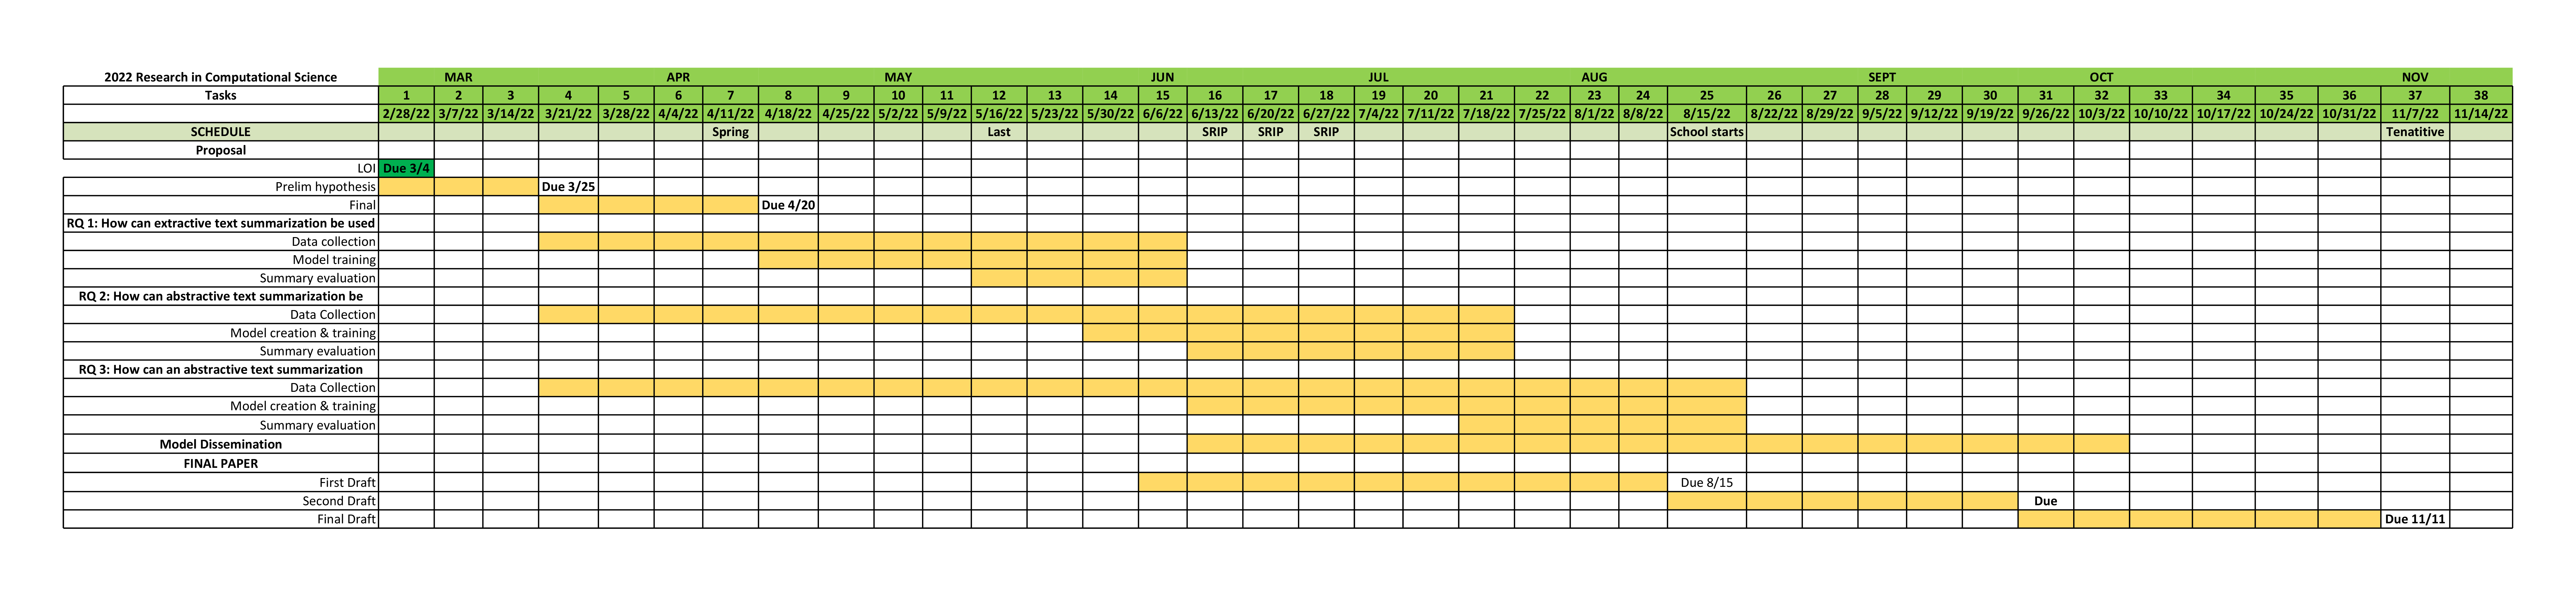
\includegraphics[scale=0.05]{images/RCompSci2022GANTTChart (1).png}
    \caption{First draft of GANTT chart}
    \label{fig:gantt}
\end{figure}

\subsection{Tuesday, March 22, 2022}
Today I wrote the intellectual merits part of my preliminary proposal and also created an outline for the rest of the proposal. I also wrote the overview, dissemination, and finished the project personnel part of my proposal.

\subsection{Wednesday, March 23, 2022}
\begin{itemize}
    \item Came up with the name of my project: Machine Learning for Research Paper Simplification (MAL-
REPS)
    \item Wrote the overview of my project
    \item Exapnded on RQ1, 2, and 3 and added them to the proposal.
    \item Rationale for MALREPS
    \item Theoretical framework (started on it)

\end{itemize}



\subsection{Thursday, March 24, 2022}
I FINISHED WRITING MY PRELIMINARY PROPOSAL TODAY AND I TURNED IT IN!!!

\subsection{Friday, March 25, 2022}
Today I watched the video \href{https://www.youtube.com/watch?v=7kLi8u2dJz0}{"What is BERT? | Deep Learning Tutorial 46 (Tensorflow, Keras & Python)"} which goes over what BERT is and how to use it.

How can similarity be captured between different words? You can look at features between different words.
\begin{enumerate}
    \item Look at various features of the input text
    \item Create vectors of the values of each feature of each input text (called a word embedding)
    \item The model figures out each feature on its own (we don't know how ML works)
    \item BERT can generate contextualized embedding (unlike something such as Word2Vec), which means that the same word used in two different contexts will generate different embedding
\end{enumerate}

\subsection{Saturday, March 25, 2022}
Today I read over the TensorFlow hub documentation for how to preprocess and use the BERT model itself to create text embeddings. There are also many other models that can be used for word embeddings, such as ulmfit, electra, gtr, and more.

I also found a pretty interesting research paper that describes when BERT was created. I will probably read this paper in the upcoming days. The paper is here \href{https://arxiv.org/abs/1810.04805}{BERT: Pre-training of Deep Bidirectional Transformers for Language Understanding
}

The BERT model source code is \href{https://github.com/google-research/bert}{here on GitHub}.

\subsection{Sunday, March 27, 2022}
Today I wrote code that is able to preprocess text and generate word embeddings using BERT from the tensorflow hub website.

\section{Week of March 28, 2022}
\subsection{Monday, March 28, 2022}
Today I watched the video \href{https://www.youtube.com/watch?v=hOCDJyZ6quA}{Text Classification Using BERT & Tensorflow | Deep Learning Tutorial 47 (Tensorflow, Keras & Python)}. Notes from my video are below:

\begin{itemize}
    \item Downsampling, take the smallest number of rows based on each category. Ex: x has 100 samples while y has 300 samples. Take 100 rows of x and 100 rows of y to train the data.
    \item sklearn.model\_selection has a function called train\_test\_split that is able to split pandas data frame into training and test data
    \item The code from this video is on \href{https://github.com/codebasics/deep-learning-keras-tf-tutorial/blob/master/47_BERT_text_classification/BERT_email_classification-handle-imbalance.ipynb}{GitHub}
    \item sklearn.metrics.pairwise has a function called cosine\_similarity that can measure the similarity between two sentences that have been turned into a vector with BERT.
    \item Metrics in ML don't actually have an effect on the model train (that works on the loss function)
    \item you can only rely on accuracy when using a BALANCED dataset
    \item Confusion matrix shows correct and wrong predictions
\end{itemize}

I sent emails to:
\begin{itemize}
    \item Mr. Miller (Leveraging BERT)
    \item Dr. Srivastava (NLP UNC)
\end{itemize}

\subsection{Tuesday, March 29, 2022}
Word2Vec is a method of turning a sentence into a sequence of numbers, because comoputers can only understand numbers. I watched the video: \href{https://www.youtube.com/watch?v=hQwFeIupNP0}{What is Word2Vec? A Simple Explanation | Deep Learning Tutorial 41 (Tensorflow, Keras & Python)}

\begin{itemize}
    \item Embeddings are created via neural networks.
    \item ``Self-supervised", meaning that there isn't necessarily a correct output
    \item Words that have a similar meaning result in similar vectors.
\end{itemize}

The way word embeddings are created:
\begin{enumerate}
    \item Take a fake problem (such as fill in a missing word in sentence--BERT)
    \item Solve it using neural network
    \item Word embedding is created as a SIDE EFFECT 
\end{enumerate}

I also began reading the research paper: \href{https://arxiv.org/pdf/2109.06838.pdf}{Employing Proverbs in Context as a Benchmark for Abstract
Language Understanding}

\begin{itemize}
    \item Email sent to Dr. Bansal (mbansal@cs.unc.edu)
    \item Email sent to Dr. Dhingra (bdhingra@cs.duke.edu)
    \item Email sent to Dr. Barzilay (regina@csail.mit.edu)
\end{itemize}

\subsection{Wednesday, March 30, 2022}
Today I prepared the Python workshop that I will be presenting to the class on Thursday (3/31). The topics that I created code for are:
\begin{itemize}
    \item Basic Python syntax
    \item data science (tables, datasets, plotting, analyzing data)
    \item sentiment analysis
    \item Classifying movie reviews
\end{itemize}

\subsection{Thursday, March 31, 2022}
Today I presented the Python workshop in class. I think that it went really well, except for a few parts where Mr. Gotwals said that R was better than Python O-O

Emails sent today:
\begin{itemize}
    \item Dr. Chaturvedi (snigdha@cs.unc.edu)
    \item Dr. Woodsend (email failure)
\end{itemize}

\subsection{Friday, April 1, 2022}
In class today, we learned about file management, UNIX commands, and how computers really work. I think that taking out ``since you're an expert, I was wondering...." makes my emails sound more professional. I also don't know whether or not keeping the line ``I would like to talk to you about my own research questions and hear your thoughts on them" is a good way to ask when emailing potential mentors.

Emails sent today:
\begin{itemize}
    \item Dr. Wiseman (swiseman@duke.edu)
    \item Dr. Wills (lisa@cs.duke.edu)
\end{itemize}

\subsection{Saturday, April 2, 2022}
Emails sent to today:
\begin{itemize}
    \item Dr. Fahlman (sef@cs.cmu.edu)
    \item Dr. Singh (singh@ncsu)
\end{itemize}





%%%%%%%%%%%%%%%%%%%%%%%%%%%%%%%%%%%%%%%%%%%%%%%%%%%%%%%%%%%%%%%%%%%%%%%%%%%%%%%%%%%
\newpage
Note: all of my sources are in Mendeley, so I don't have a bibliography here.




\end{document}

\begin{comment}
%Sample LaTeX Code
    % \bibitem{giusti}
    % Giusti, Santochi, \emph{Tecnologia Meccanica e Studi di Fabbricazione}. Casa Editrice Ambrosiana, Seconda Edizione
    
    
    % \begin{figure}[H]\centering
    % \includegraphics[scale=0.5]{weintrop.jpg}
    % \caption{Weintrop's Taxonomy}
    % \label{fig:weintrop}
    % \end{figure}

\end{comment}
